
\chapter{提案手法}
\label{chap:proposed}

%----------------------------------------------
\section{まえがき}
%----------------------------------------------
前章では,\red{音響信号のBSSにおいて重要な}FDICA\blue{に伴い生じる}\red{の}パーミュテーション問題\blue{と従来の深層}\red{について詳しく述べた.また,音源モデルに基づきパーミュテーション問題を回避する手法や,近年提案された深層}パーミュテーション解決法について説明した.
\red{さらに,既存の深層パーミュテーション解決法では,音源数$N$の増加に伴ってアルゴリズムが極端に複雑になってしまう課題について述べた.}
本章では,\blue{組み合せ爆発を起こすことのない,DNNを用いたデータ駆動型パーミュテーション解決法を新たに提案する.}
\red{音源数$N$が増加した場合でもアルゴリズムが複雑化することのない深層パーミュテーション解決法を新たに提案する.}
\blue{{\ref{sec:moti}}節では,IVAやILRMAのようなブラインド(教師無し)なパーミュテーション解決法における課題と従来の深層パーミュテーション解決法における課題を述べ,データ駆動型の教師ありパーミュテーション解決法を新たに提案する動機について明らかにする.}
\red{まず\ref{sec:moti}節では,BSSにおいて深層学習を用いてパーミュテーション問題の解決を目指す動機について述べる.}
\ref{sec:in-out}節及び\ref{sec:model}節で\red{は},\blue{提案}\red{本論文で提案する深層}パーミュテーション解決法\blue{における}\red{の}DNNモデルの入出力及び\red{ネットワーク}構造を\red{それぞれ}説明する.
\ref{sec:loss}節及び\ref{sec:maj}節では,誤差逆伝播に用いる損失\red{関数}の取り方と\blue{パーミュテーション行列の並び替えに用いる}\red{パーミュテーション行列を正確に推定するモデルを学習するための}\blue{ラベルの取得方法}\red{入力データ及び正解データ(ラベル)の取得方法}を\red{それぞれ}説明する.
\ref{sec:3matome}節で本章のまとめを述べる.

%----------------------------------------------
\section{動機}
\label{sec:moti}
%----------------------------------------------
%%%%%%%%%%%%%%%%%%%%%%%%%%%%
\begin{figure}[t]
    \begin{center}
        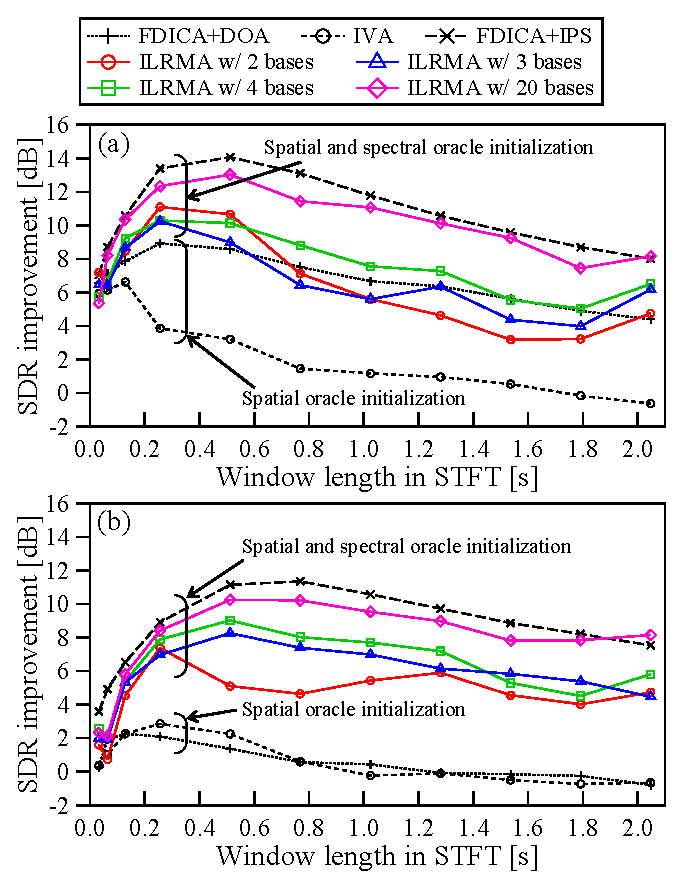
\includegraphics[width=0.8\columnwidth]{figures/SpeechE2AJR2_opt12+note.eps}
    \end{center}
    \vspace{-8pt}
	\caption{Average source separation results for speech signals using random initialization: (a) E2A (\red{$T_{60} = 300$~ms}) and (b) JR2 (\red{$T_{60}=470$~ms}) impulse responses. \red{For details of this figure, see~\cite{EU}.}}
	\label{fig:kitamura_es}
\end{figure}
%%%%%%%%%%%%%%%%%%%%%%%%%%%%

文献~\cite{EU}では,\red{IVAやILRMAに基づく}BSSのSTFTにおける最適な\blue{窓長を}\red{短時間区間長(窓長)$Q$について}実験的に\blue{検討}\red{調査}している.
Fig.~\ref{fig:kitamura_es}(b)は,文献~\cite{EU}の実験結果の図を引用したものである.\red{詳しい実験条件等は文献\cite{EU}を参照されたい.}縦軸は信号対歪み比(source-to-distortion ratio: SDR)\cite{BSSEval}の改善量であり,これは即ち\blue{分離性能}\red{音源分離の性能}を表している.
この結果より,IVA及びILRMAでは,残響\blue{状態}\red{時間が}\blue{{$T_{60} = $}}$470~\mathrm{ms}$\blue{の条件}\red{という比較的残響の強い条件}では\red{,IVAもILRMAも高精度な音源}分離に失敗していることが分かる.
一方で,FDICAに対して,音源信号$\bm{s}_{ij}$を用いる理想的なパーミュテーション解決法(ideal permutation solver: IPS)を適用した結果\red{(すなわちFDICAの達成しうる限界性能)}では10~dB以上のSDRの改善を達成している.
この事実は,高残響下での\blue{音声混合信号}\red{音声信号の混合という難しい観測条件}であっても,$\hat{\bm{W}}_i$\blue{はFDICAで正確に推定でき,}\red{の推定自体(すなわち周波数ビン毎のBSS)はFDICAでも高精度に実現できていることを示している.すなわち,残る課題は推定信号$\bm{y}_{ij}$を正しい順番に並び変えるパーミュテーション問題の解決(}
$\bm{P}_i^{-1}$の\blue{推定のみ失敗していることを示している.}
\red{推定)のみであることを示唆している.}
また,\red{\ref{sec:DNNs}節で述べた通り,}従来の深層パーミュテーション解決法では,\blue{全周波数帯域中の局所的な狭帯域のおける}\red{サブバンド内の}パーミュテーション問題\blue{の解決を全時間方向と全周波数方向に行う際に,}
\red{を解決する際に,}\blue{ある}参照周波数\red{ビン}に対して\blue{同一か否かで音源を判断しているため,3音源以上の分離等の拡張性に欠ける.}
\red{その他の周波数ビンの推定信号成分が同一音源の成分か否かの2クラス分類問題をDNNで予測している.音源数が$N=2$であれば,この「同一音源の成分か否か」の2クラス分類はすなわち「どちらの音源の成分か」に一致するが,音源数が$N\geq 3$となった場合は,
「同一音源の成分ではない」とDNNが判断した場合にその成分がどの音源の成分かが確定しない.従って,この場合に各推定成分がどの音源に対応するかを確定させるためには,先の2クラス分類DNNモデルを音源数$N$個の中から2つ選ぶ組み合わせ数(${}_N C_2$)分適用せねばならず,
さらに後段のサブバンド間のパーミュテーション問題の解決(全サブバンドのスティッチング)の処理を考えると,そのアルゴリズムは非常に複雑・煩雑になってしまう.
}

そこで,本論文では,簡潔なアルゴリズムでパーミュテーション問題を正確に解くことに焦点を当て,新しい\blue{DNNに基づくデータ駆動型(教師あり)パーミュテーション解決法}\red{深層パーミュテーション解決法}を提案する.
以後,本論文では,提案するパーミュテーション問題の解決法が実現可能かどうかを\blue{判断するために,}\red{判断するための基礎的な調査として,}FDICAを適応した後の分離信号\blue{に}\red{を}模倣した人工データと
実際の\blue{音声データ}\red{音響信号}を用いてパーミュテーション問題の\blue{解決を考える}\red{解決性能を実験的に調査する}.
\blue{この際,音源数{$N=2$}及びチャネル数{$M=2$}と仮定し,実験を行う.}
\red{提案手法は,音源数$N$の増加に対してアルゴリズムが極端に複雑化しない手法として提案するが,本論文は基礎的な実験に終始するため,音源数及びチャネル数が$N=M=2$の状況のみを取り扱う.$N\geq 3$以上の条件での調査については今後の課題となる.}

\blue{提案する}\red{本論文で提案する深層}パーミュテーション解決法\blue{の概要}\red{を適用する処理の概要}は以下の通りである.
\red{
\begin{enumerate}
\renewcommand{\labelenumi}{(\alph{enumi})}
    \item \red{パーミュテーション問題が未解決の状態である推定信号{$\bm{Y}_1$及び$\bm{Y}_2$}に対し,両信号のパワー比に基づく正規化\cite{Permutation_solverBSS}を施す}
    \item \red{正規化された両信号のスペクトログラムから,ある時間フレーム$j$とその前後$j\pm\beta$の時間フレームの部分的なスペクトログラムを抽出し,時間フレーム$j$を中心とした局所時間振幅スペクトログラムを両信号で構成する}
    \item \red{両信号の局所時間振幅スペクトログラムをベクトル化し,DNNに入力する.}
    \item \red{DNNは入力ベクトル中の$\bm{Y}_1$及び$\bm{Y}_2$の正規化局所時間振幅スペクトログラムの各周波数ビンの成分がそれぞれどの音源信号に属するかを分類問題として予測し,周波数毎及び音源毎の確率値をまとめたベクトルを出力する}
    \item \red{(b)--(d)の処理を全時間フレームに対して適用し,時間フレーム毎の確率値ベクトルを取得する}
    \item \red{全時間フレームの確率値ベクトルを用いて時間方向に多数決処理を適用し,全時間フレーム共通の(1本の)確率値ベクトルを得る}
    \item \red{確率値ベクトルから周波数毎のパーミュテーション行列$\bm{P}_i$の推定値$\hat{\bm{P}}_i$を構成する}
    \item \red{式(\ref{eq:z})よりパーミュテーション問題が解決された分離信号を得る}
\end{enumerate}
}
\blue{提案するパーミュテーション解決法では,全周波数成分を持ったミニ振幅スペクトログラムに対して,どの音源の成分が入っているかをDNNで予測し,その予測結果に基づいてパーミュテーション解決を行う.また,}
\red{上記の処理の詳細やDNNの学習方法については,次節以降で詳しく述べる.}
\blue{DNNには大量の学習用データが必要であるが,IPSで理想的にパーミュテーション解決された分離信号{$\bm{Z}_n$}を周波数毎にランダムにシャッフルすることで,容易かつ大量に生成することができる.}
%----------------------------------------------
\section{DNNの入出力}
\label{sec:in-out}
%----------------------------------------------

\blue{観測された混合信号{$\bm{X}_n$}にFDICAを適用すると,} \red{提案する深層パーミュテーション解決法で用いられるDNNは複数の全結合層からなる多層パーセプトロン(multi-layer perceptron: MLP)を想定している.
MLPの入出力はあらかじめ決められた次元数のベクトルでなければならない.今,観測信号$(\bm{X}_1, \bm{X}_2)$にFDICAを適用した場合を考える.FDICAからは,
}パーミュテーション問題\blue{が生じた分離信号{$\bm{Y}_n$}が得られる.}
\red{が発生した状態の推定信号$(\bm{Y}_1, \bm{Y}_2)$が得られる.}
\blue{DNNへの入力は,各分離信号のパワースペクトログラム成分を全ての分離信号のパワースペクトログラム成分で割った値を用いる.
即ち,2音源の場合DNNの入力に用いる信号成分は次のようになる.}
\red{ここで,同一音源に属する成分の相関を強調するため,推定信号$(\bm{Y}_1, \bm{Y}_2)$のパワースペクトラム$(|\bm{Y}_1|^{.2}, |\bm{Y}_2|^{.2})$の比率に変換する正規化\cite{Permutation_solverBSS}を施す.この処理は次式で表される.}
\begin{align}
    \red{\overline{\bm{Y}}_1 = \frac{|\bm{Y}_1|^{.2}}{|\bm{Y}_1|^{.2}+|\bm{Y}_2|^{.2}}} \in [0,1]^{I \times J}\\
    \red{{\overline{\bm{Y}}_2 = \frac{|\bm{Y}_2|^{.2}}{|\bm{Y}_1|^{.2}+|\bm{Y}_2|^{.2}}} \in [0,1]^{I \times J}}
\end{align}
ここで,\blue{DNNの入力に用いる値をそれぞれ{$\widehat{\bm{Y}}_1~\in \mathbb{R}_{\geq 0}^{I \times J}$,$\widehat{\bm{Y}}_2 ~\in \mathbb{R}_{\geq 0}^{I \times J}$}とする.}
\red{行列に対する絶対値記号は要素毎の絶対値,行列やベクトルに対するドット付き指数乗は要素毎の指数乗,及び行列間のベクトルは要素毎の商を示している.}
\blue{この時,{$i = 1,\ldots,I$及び$j = \tau,\ldots,J-\tau$}はそれぞれ全周波数帯域の周波数ビン及び時間フレームのインデクスである.DNNの入力にはミニ振幅スペクトログラムを用いるので,元のスペクトログラムの値からはみ出ることがないように{$j$}の範囲を限定的にしている.
ここで,行列の {$|\cdot|^{.2}$} は,要素ごとの絶対値の二乗を示す.時間フレーム{$j$}における分離信号を次式で表す.}
\red{このような正規化は,文献\cite{Permutation_solverBSS}で詳しく解析されているように同一音源に属する成分の相関を強調させる利点があるだけでなく,推定信号の値が区間$[0,1]$の範囲に限定されることから,DNNの学習を安定させる効果も期待できる.}
\red{次に,推定信号の正規化振幅スペクトログラム$(\overline{\bm{Y}}_1, \overline{\bm{Y}}_2)$から,Fig.~\ref{fig:make_minispec}に示すように,時間フレーム$j$を中心とする局所時間振幅スペクトログラムを抽出する.この処理は次式で表される.}
%%%%%%%%%%%%%%%%%%%%%%%%%%%%
\begin{figure}[t]
    \begin{center}
        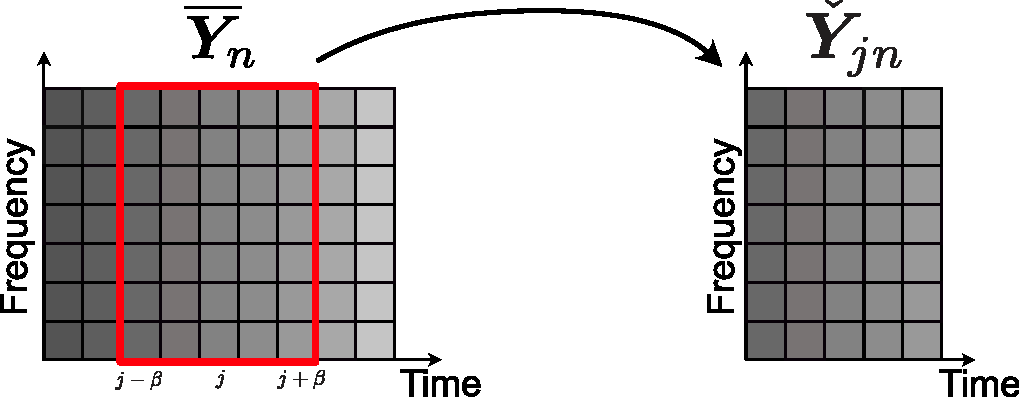
\includegraphics[width=0.95\columnwidth]{figures/make_minispec.pdf}
    \end{center}
    \vspace{-8pt}
	\caption{Extraction of local-time-frame amplitude spectrogram.}
	\label{fig:make_minispec}
\end{figure}
%%%%%%%%%%%%%%%%%%%%%%%%%%%%
\red{
    \begin{align}
        \check{\bm{Y}}_{j1} &= [ \overline{\bm{y}}_{(j-\beta)1}, \overline{\bm{y}}_{(j-\beta+1)1}, \cdots, \overline{\bm{y}}_{(j-1)1}, \overline{\bm{y}}_{j1}, \overline{\bm{y}}_{(j+1)1}, \cdots, \overline{\bm{y}}_{(j+\beta)1}  ] \in [ 0, 1 ]^{I\times (2\beta+1)} \label{eq:y_check1}\\
        \check{\bm{Y}}_{j2} &= [ \overline{\bm{y}}_{(j-\beta)2}, \overline{\bm{y}}_{(j-\beta+1)2}, \cdots, \overline{\bm{y}}_{(j-1)2}, \overline{\bm{y}}_{j2}, \overline{\bm{y}}_{(j+1)2}, \cdots, \overline{\bm{y}}_{(j+\beta)2}  ] \in [ 0, 1 ]^{I\times (2\beta+1)} \label{eq:y_check2}
    \end{align}
}
%%%%%%%%%%%%%%%%%%%%%%%%%%%%
\begin{figure}[t]
    \begin{center}
        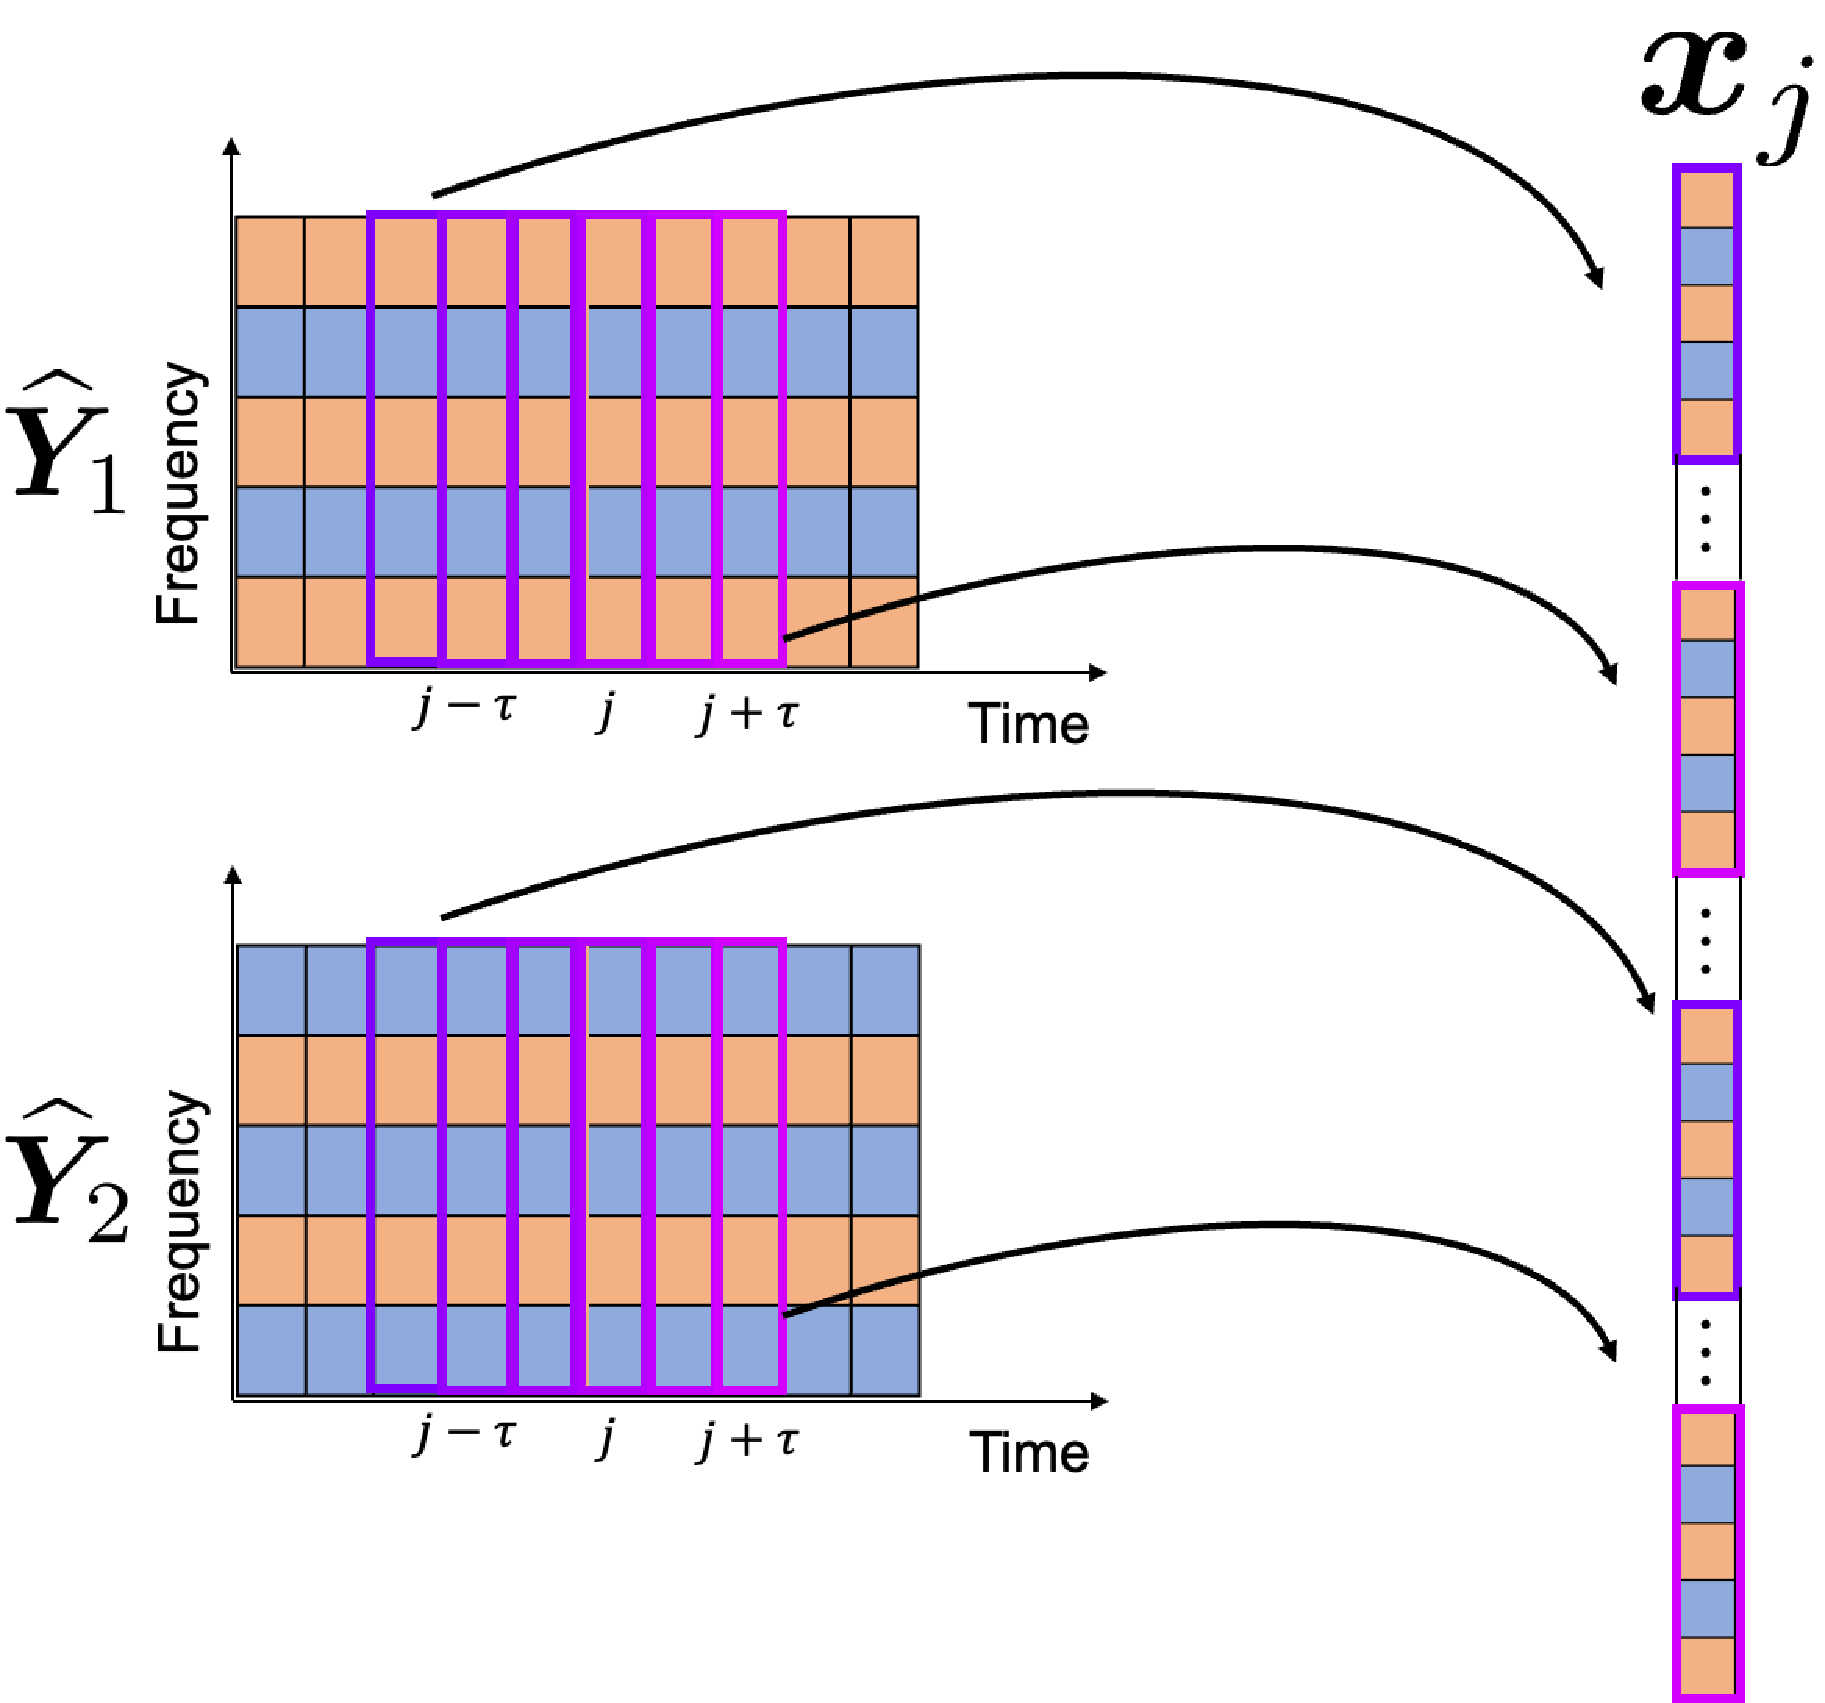
\includegraphics[height=0.8\columnwidth]{figures/DNN_input.pdf}
    \end{center}
    \vspace{-8pt}
	\caption{Input vector of DNN.}
	\label{fig:DNN_input}
\end{figure}
%%%%%%%%%%%%%%%%%%%%%%%%%%%%
\red{ここで,$\overline{\bm{y}}_{jn}\in [0,1]^{I}$は正規化振幅スペクトログラム$\overline{\bm{Y}}_n$の$j$列目の列ベクトル(時間フレーム$j$の正規化振幅スペクトル)を表す.
また,$\beta$(0以上の整数)は時間フレーム$j$の近傍時間フレームをどの程度DNNに入力するかを決めるパラメータである.}
\blue{DNNの入力として与える情報}\red{提案手法では,DNNの入力ベクトル}は,\blue{{$j$}近傍の時間フレームの列ベクトルを結合したベクトルとする.}
\red{式(\ref{eq:y_check1})及び(\ref{eq:y_check2})で得られる両信号の正規化局所時間振幅スペクトログラム$(\check{\bm{Y}}_{j1}, \check{\bm{Y}}_{j2})$をFig.~\ref{fig:DNN_input}のように一次元に整形(ベクトル化)したベクトルである.}
\blue{これを{$\bm{x}_j$}とおくと,次式のように構成される.}
\red{入力された行列をベクトル化する処理を$\mathrm{vec}(\cdot)$と表記すると,DNNの入力ベクトルは次式となる.}
\begin{align}
    \red{\bm{d}_j = \begin{bmatrix}
        \mathrm{vec}( \check{\bm{Y}}_{j1} ) \\
        \mathrm{vec}( \check{\bm{Y}}_{j2} )
      \end{bmatrix}
    \in [0,1]^{2I(2\beta+1)}}
\end{align}

\red{DNNによる予測は次式で表される.}
\begin{align}
    \red{\hat{\bm{l}}_j = \mathrm{DNN}(\bm{d}_j) \in [ 0, 1 ]^{2I}}
\end{align}
%%%%%%%%%%%%%%%%%%%%%%%%%%%%
\begin{figure*}[!t]
    \centering
    \subfloat[Calculatation of predicted permutation matrix.]{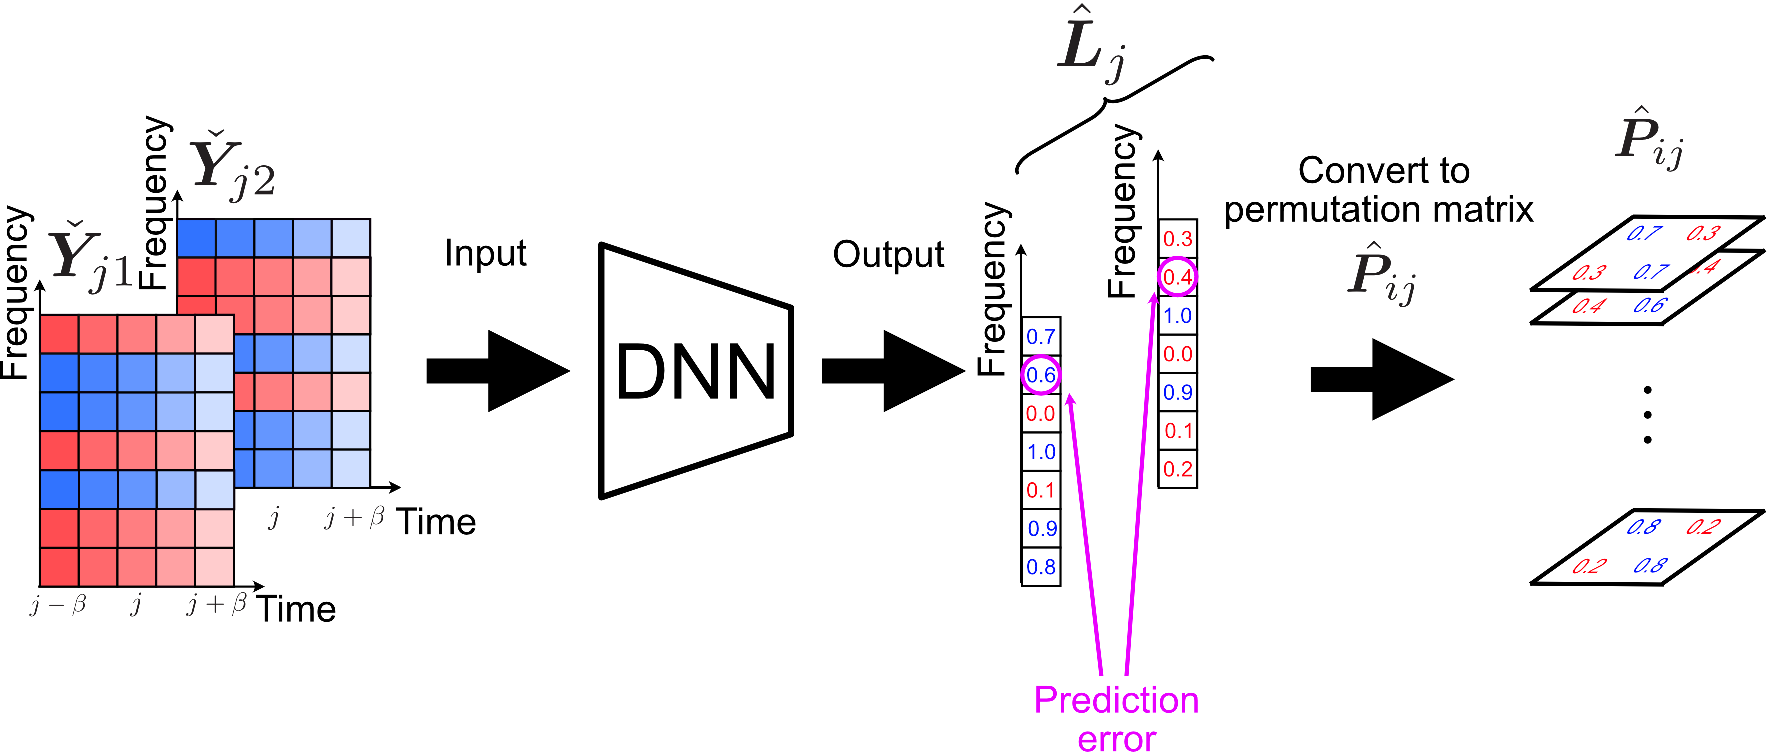
\includegraphics[clip, width=5.0in]{figures/cal_loss1.pdf}
    \label{fig:loss_process1}}
    \\
    \subfloat[Calculation of MSE with PIT]{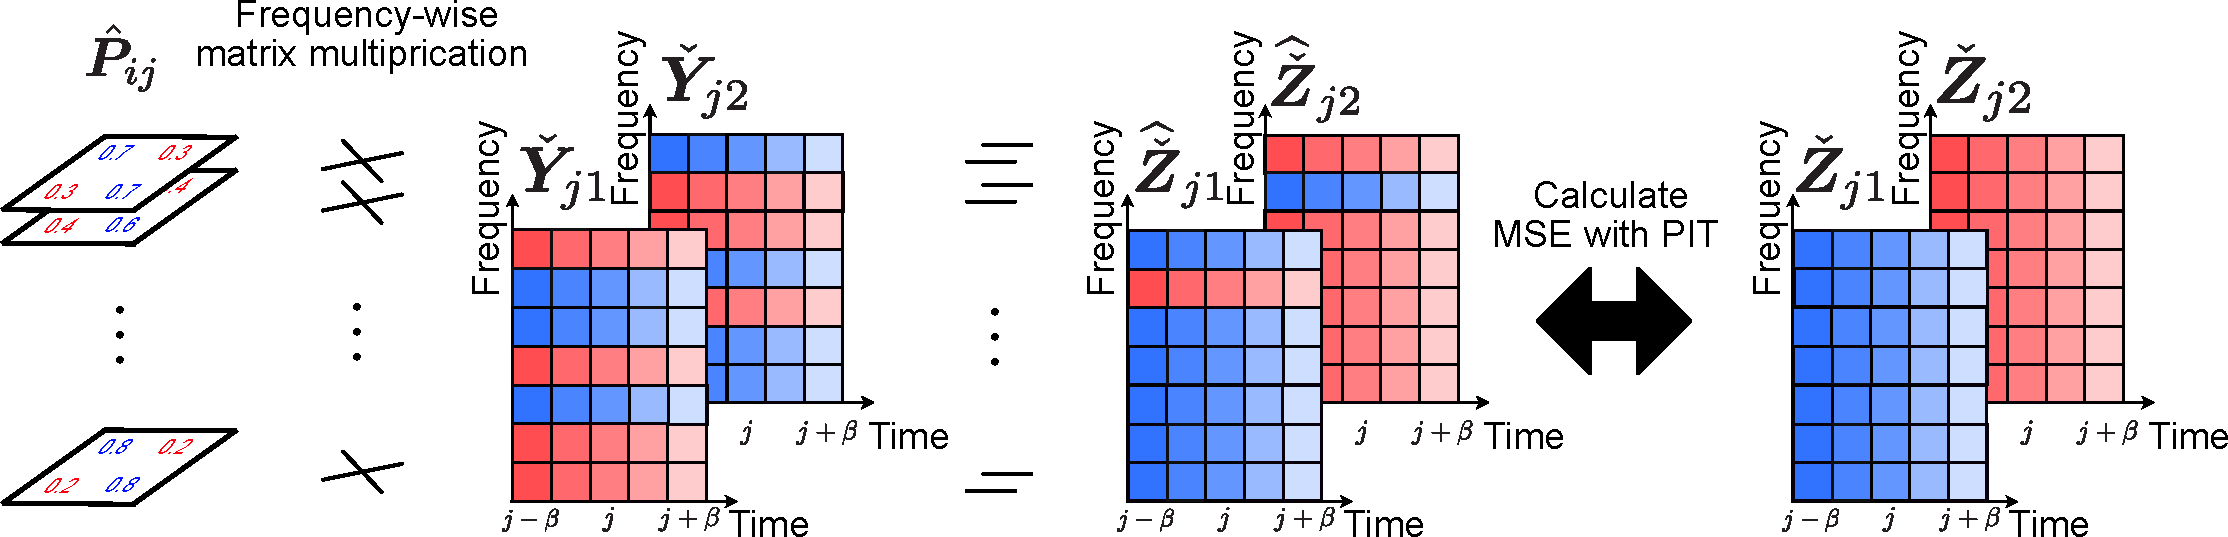
\includegraphics[clip, width=5.0in]{figures/cal_loss2_v2.pdf}
    \label{fig:loss_process2}}  
    \caption{Process of calculating predicted permutation matrix and loss function value.}
    \label{fig:loss}
\end{figure*}
%%%%%%%%%%%%%%%%%%%%%%%%%%%%
\blue{DNNが出力する予測は{$\bm{L} ~\in \mathbb{R}_{[0,1]}^{2 \times I}$}であり,確率値を示す.
{$\bm{L}$}の1行目には,各周波数成分における音源1である確率値,2行目には,各周波数成分における音源2である確率値が代入される.}
\red{ここで,$\hat{\bm{l}}_j = [ \hat{l}_{11j}, \hat{l}_{21j}, \cdots, \hat{I1j}, \hat{12j}, \hat{22j}, \cdots, \hat{I2j} ]^\mathrm{T}$は出力である予測ベクトルを表す.
入力されたベクトルを行列化する処理を$\mathrm{mat}(\cdot)$と表記すると,予測ベクトルは次式で再成型される.
\begin{align}
  \hat{\bm{L}}_j = \mathrm{mat}(\hat{\bm{l}}_j) \in [0, 1]^{I \times 2}
\end{align}
再成型された行列$\hat{\bm{L}}_j$はFig.~\ref{fig:loss_process1}に示すように,2つのパーミュテーション問題が生じている入力信号$(\check{\bm{Y}}_{j1}, \check{\bm{Y}}_{j2})$の各周波数成分のそれぞれが
「1番目の音源の成分である確率$l_{i1}$」と「2番目の音源の成分である確率$l_{i2}$」を$\bm{d}_j$から予測したものと定義し,提案手法ではこの定義に基づいて正確な予測ができるDNNを学習する.
ここで,$(l_{i1}, l_{i2})$は離散確率値であるため$l_{i1}+l_{i2}=1$を満たし,それらの予測値である$(\hat{l}_{i1j}, \hat{l}_{i2j})$もまた$\hat{l}_{i1j}+\hat{l}_{i2j}=1$を満たすようにDNNの中で制約する必要がある.
この制約は次節で述べる通り,softmax関数を用いて実現できる.また,詳細は後述するが,パーミュテーション問題の解は時間方向には変化しない(式(\ref{eq:w_fdica})における$\bm{P}_i$は時間フレーム$j$によらない時不変行列である)ため,
様々な局所時間振幅スペクトログラムの入力$\bm{d}_j$の予測結果$\hat{\bm{L}}_j$を$j$に関して多数決処理することで,より精度の高い予測である予測結果$\hat{\bm{L}}$(この結果は$j$によらない)を生成できる.
}

\red{
重要なこととして,確率値$(l_{i1}, l_{i2})$は式(2.27)で述べたパーミュテーション行列それ自身と本質的に等価である.従って,DNNの予測結果である$(\hat{l}_{i1}, \hat{l}_{i2})$から推定パーミュテーション行列を次式で構成できる.
\begin{align}
  \hat{\bm{P}}_{i} = 
  \begin{bmatrix}
    \hat{l}_{i1} & \hat{l}_{i2} \\
    \hat{l}_{i2} & \hat{l}_{i1}
  \end{bmatrix} \label{eq:estPermMat}
\end{align}
ここで,$\hat{l}_{i1}$及び$\hat{l}_{i2}$は$\hat{\bm{L}}$の要素である.正解のパーミュテーション行列は順列を並び替える行列であるため,$N=2$の場合は式(\ref{eq:permu_mat_2dim})のいずれかとなる.
推定パーミュテーション行列$\hat{\bm{P}}_{i}$は式\eqref{eq:estPermMat}であるため,予測が不完全であれば$\bm{I}$又は$\bm{1}-\bm{I}$にはならない可能性があるが,
それでも$\hat{l}_{i1}+\hat{l}_{i2}=1$を満たすため,二重確率行列(doubly stochastic matrix: DSM)であることがわかる.
また,Birkhoff--von Neumannの定理を考慮すると,パーミュテーション問題の発生している入力データからDSMを予測する提案手法のDNNは,
考えうる全てのパーミュテーション行列に対する凸結合係数を推定していることになる.
即ち,考えうるパーミュテーション行列の中でどの行列が正解かという確信度を予測していると解釈することもできる.
}

%----------------------------------------------
\clearpage
\section{DNNの構造}
\label{sec:model}
%----------------------------------------------
%%%%%%%%%%%%%%%%%%%%%%%%%%%%
\begin{figure}[t]
    \begin{center}
        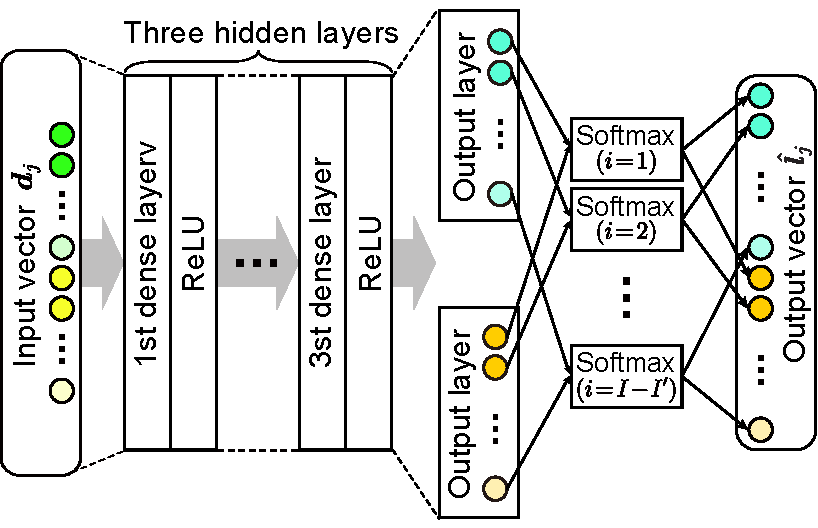
\includegraphics[width=0.8\columnwidth]{figures/architecture_DNN.pdf}
    \end{center}
    \vspace{-8pt}
	\caption{DNN architecture.}
	\label{fig:Dnnmodel}
\end{figure}
%%%%%%%%%%%%%%%%%%%%%%%%%%%%

Fig.~\ref{fig:Dnnmodel}に提案深層パーミュテーション解決法で用いるDNNの構造を示す.
このDNNは,入力層,隠れ層3層,及び出力層の計5層\red{の全結合層(dense layer)}からなる\blue{全結合構成}\red{MLP}となっており,\blue{1~5番目の隠れ層には}\red{隠れ層の1層目から3層目には非線形関数として}rectified linear unit (ReLU)~\cite{relu} 関数
\red{を用いている.
また,3層目の隠れ層から出力層に変換する際には,Fig.~\ref{fig:Dnnmodel}に示すように2つの$I$次元ベクトルに分岐させている.この時の各ベクトルへの変換パラメータは独立している\footnote{すなわち,$2I$次元への全結合層による変換と同様であるが,明示的に分岐させて定義している.}.
その後,2つの$I$次元の同一インデクスの要素に対してsoftmax関数を適用することで,予測ベクトルの全要素が閉区間$[0,1]$内の値かつ同一インデクスの要素の和が1となることを保証している.
これは,前節で説明した$\hat{l}_{i1}+\hat{l}_{i2}=1$の制約を保証することに対応し,これによって予測ベクトルを確率値としてみなすことが可能となる.}
\blue{最終隠れ層にはsoftmax関数を適用している.}
\blue{各隠れ層の次元数は全て,4096である.}

%----------------------------------------------
\section{\red{DNN学習時の損失関数}}
\label{sec:loss}
%----------------------------------------------
\red{DNNの学習は,何らかの損失関数を定義しその値を最小化するパラメータを誤差逆伝播により推定する処理となる.提案手法のDNNは\ref{sec:in-out}節で述べた通り,入力データから周波数毎の正しい音源パーミュテーションを予測するモデルである.
これは(音源数が$N=2$であれば)$(l_{i1}, l_{i2})$の2クラス分類器であるため,softmax関数を用いて各クラスへの確率値を出力している.
通常,多クラス分類器の損失関数には,カテゴリカル分布\footnote{多項分布における試行回数を1回とした際の分布である.}の負対数尤度関数であるカテゴリカル交差エントロピー(categorical cross entropy: CCE)を用いることで,DNNの学習を最尤推定の枠組みで行うことができる.
しかしながら,提案手法の深層パーミュテーション解決法の本来の目的は,全周波数ビンにおいてパーミュテーション行列を正確に予測することではなく,分離信号$(\bm{Z}_1, \bm{Z}_2)$を正確に予測することである.
例えば,推定信号$(\bm{Y}_1, \bm{Y}_2)$のどちらにもエネルギーがほとんど無いような周波数ビンは,実際は誤った分離信号の順序となっていても得られる分離信号$(\bm{Z}_1, \bm{Z}_2)$の音源分離精度には影響しない.
もしCCEでDNNの損失関数を定義すると,このようなエネルギーが少ない(音源分離にとって重要ではない)周波数ビンのパーミュテーション予測精度と,
大きなエネルギーを有する(音源分離にとって重要な)周波数ビンの予測精度が等しい重要度で扱われることになるため,音源分離性能向上の妨げとなる可能性がある.}

\red{そこで提案手法では,下記で説明する通り,DNNで予測された音源パーミュテーションに基づいて推定信号$(\bm{Y}_1, \bm{Y}_2)$を並び替えた予測分離信号$(\hat{\bm{Z}}_1, \hat{\bm{Z}}_2)$と正解の分離信号$(\bm{Z}_1, \bm{Z}_2)$の間の平均二乗誤差(mean squared error: MSE)を示す.}

\red{Fig.~\ref{fig:loss_process1}に損失関数の計算の処理の流れを示す.まず,予測結果に対応する行列$\hat{\bm{V}} \in \mathbb{R}^{R\times C}$とラベルに対応する行列$\bm{V} \in \mathbb{R}^{R\times C}$の間のMSEを次式で定義する.}
\red{
\begin{align}
    \mathrm{MSE}(\hat{\bm{V}}, \bm{V}) &= \frac{ 1 }{ RC } \| \hat{\bm{V}} - \bm{V} \|_\mathrm{Fr}^2 \\
    &= \frac{ 1 }{ RC } \sum_{r, c} \left( \hat{v}_{rc} - v_{rc} \right)^2 \label{eq:mseLoss}
\end{align}
ここで,$\hat{v}_{rc}$及び$v_{rc}$はそれぞれ行列$\hat{\bm{V}}$及び$\bm{V}$の要素,$r = 1, 2, \cdots, R$及び$c = 1, 2, \cdots, C$はそれぞれ行列$\hat{\bm{V}}$及び$\bm{V}$の行と列のインデクス,$\|\cdot\|_\mathrm{Fr}$はFrobeniusノルムである.
次に,Fig.~\ref{fig:loss_process1}に示すように,DNNの入力である正規化局所時間振幅スペクトログラム$(\check{\bm{Y}}_{j1}, \check{\bm{Y}}_{j2})$に対する予測結果$\bm{L}_j$と式(\ref{eq:estPermMat})を用いて,
($j$を中心とする局所時間フレームの)推定局所時間パーミュテーション行列$\hat{\bm{P}}_{ij}$を構成する.また,Fig.~\ref{fig:loss_process2}に示すように,式(\ref{eq:w_fdica})で音源パーミュテーションを並び替えた予測分離信号$(\widehat{\check{\bm{Z}}}_{j1}, \widehat{\check{\bm{Z}}}_{j2})$を求める.
さらに,この予測分離信号に対する正解ラベル(Fig.~\ref{fig:make_minispec}と同様の手順で,分離信号$(\bm{Z}_1, \bm{Z}_2)$から$j$を中心とする局所時間フレームの局所時間振幅スペクトログラムを抽出した行列)を$(\check{\bm{Z}}_{j1}, \check{\bm{Z}}_{j2})$と定義する.
これらの信号と式\eqref{eq:mseLoss}を用いて,前述の誤差関数$\mathcal{L}$は,$(\widehat{\check{\bm{Z}}}_{j1}, \widehat{\check{\bm{Z}}}_{j2})$及び$(\check{\bm{Z}}_{j1}, \check{\bm{Z}}_{j2})$間のMSEとして次式で表せる.
\begin{align}
    \mathcal{L} &= \mathrm{MSE}(\widehat{\check{\bm{Z}}}_{j1}, \check{\bm{Z}}_{j1}) + \mathrm{MSE}(\widehat{\check{\bm{Z}}}_{j2}, \check{\bm{Z}}_{j2}) \label{eq:dnnLossWithoutPit}
\end{align}
}
\red{但し,パーミュテーション問題の解決は全周波数で推定音源成分を正しく並び替えることだけが目標であり,並び替えた後の分離信号そのものの順序は予測の対象としない.
すなわち,深層パーミュテーション解決法を適用した結果が,$(\bm{Z}_1, \bm{Z}_2)$及び$(\bm{Z}_2, \bm{Z}_1)$のどちらの順序で出力されようとも構わない.
式\eqref{eq:dnnLossWithoutPit}で損失関数を定義した場合,分離信号は必ず$(\bm{Z}_1, \bm{Z}_2)$という順序で予測することをDNNに強いているため,
この問題を解消するために順序不変学習(permutation invariant training: PIT)\cite{PIT}を導入する.具体的には,損失関数を次式で定義する.
\begin{align}
  \mathcal{L} &= \min \left( \mathrm{MSE}(\widehat{\check{\bm{Z}}}_{j1}, \check{\bm{Z}}_{j1}) + \mathrm{MSE}(\widehat{\check{\bm{Z}}}_{j2}, \check{\bm{Z}}_{j2}),  \mathrm{MSE}(\widehat{\check{\bm{Z}}}_{j1}, \check{\bm{Z}}_{j2}) + \mathrm{MSE}(\widehat{\check{\bm{Z}}}_{j2}, \check{\bm{Z}}_{j1}) \right) \label{eq:dnnLossWithPit}
\end{align}
ここで,$\min (\cdot, \cdot)$は複数のスカラー引数の中で最小値を返す処理を表す.この関数の誤差逆伝播は自動微分により実装される.このように,PITを導入することで,周波数ビン間のパーミュテーション問題さえ解決されれば良く分離信号そのものの出力の順序には依存しないような学習が可能となる.
}

%----------------------------------------------
\section{\red{学習済のDNNのテストデータへの適用}}
\label{sec:maj}
%----------------------------------------------
%%%%%%%%%%%%%%%%%%%%%%%%%%%%
\begin{figure}[t]
    \begin{center}
        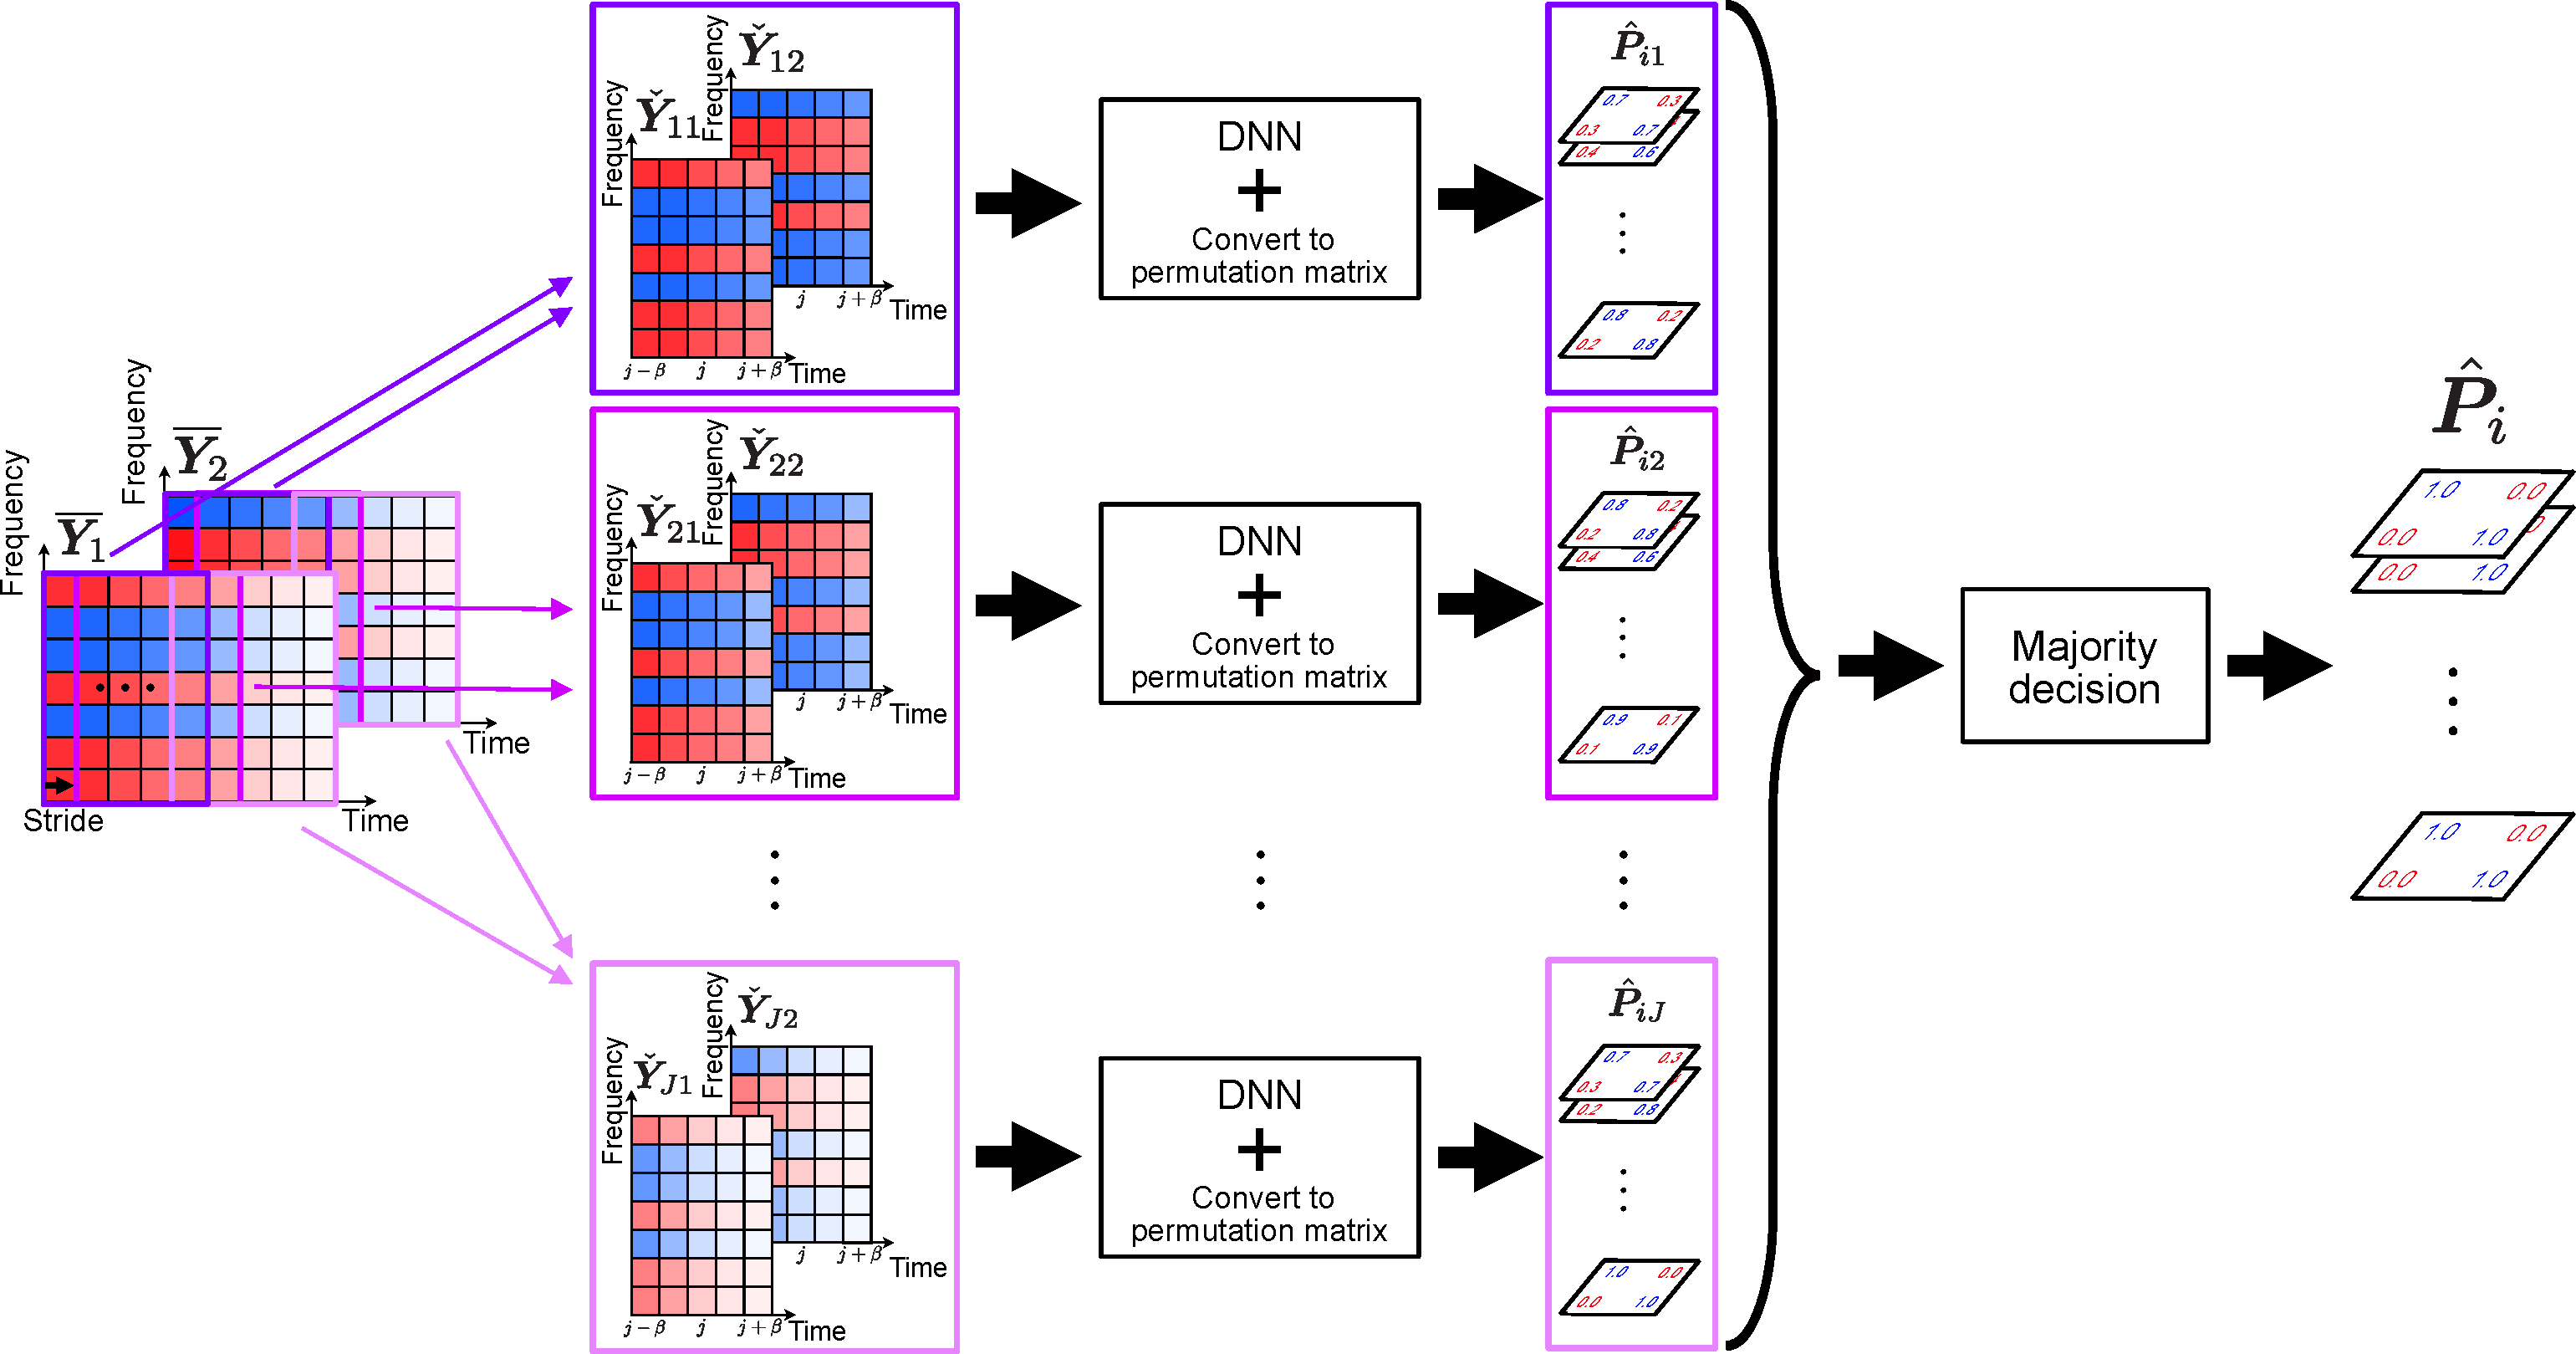
\includegraphics[width=1.0\columnwidth]{figures/majority.pdf}
    \end{center}
    \vspace{-15pt}
	\caption{DNN predictions for all local-time-frame amplitude \red{spectrograms} and their majority decision.}
	\label{fig:majority}
	\vspace{-8pt}   % キャプションと本文の間隔微調整用クトル
\end{figure}
%%%%%%%%%%%%%%%%%%%%%%%%%%%%
\blue{音声信号は本来,無音区間が多く存在することから,一定区間の長さの成分を持つ{$\widehat{\bm{Y}}_1$や$\widehat{\bm{Y}}_2$}はほぼ零ベクトルになる可能性があり,その場合DNNの予測は不安定になる.}
\blue{この問題に対処するために,Fig.~{\ref{fig:majority}}に示すように,長さ{$2\tau+1$}の入力ベクトルをストライド幅1でシフトさせて,全時間フレームに対してDNNの予測処理を走査する.}
\red{DNN学習後は,提案手法である深層パーミュテーション解決法をFDICA等の推定信号$(\bm{Y}_1, \bm{Y}_2)$に適用することができる.
このテストデータへの適用時においては,より高精度にパーミュテーション問題を解決をするために,次に示す2つの処理を施す.
\begin{enumerate}
\renewcommand{\labelenumi}{(\alph{enumi})}
  \item FDICA等で実現される周波数ビン毎のBSSが完全に達成されているならば,推定すべきパーミュテーション行列$\bm{P}_i$は0及び1の要素を持つバイナリ行列であるため,推定局所時間パーミュテーション行列$\hat{\bm{P}}_{ij}$もバイナリ行列に変換する
  \item FDICA等の時不変な分離行列$\bm{W}_i$を推定するBSSにより生じるパーミュテーション問題は,時間フレーム方向には一定である($\bm{P}_i$は$j$に非依存)ため,推定局所時間パーミュテーション行列$\hat{\bm{P}}_{ij}$を時間方向に多数決処理し,時不変な行列$\hat{\bm{P}}_{i}$に変換する
\end{enumerate}}

\red{上記(a)については,次式でバイナリ行列への変換処理を実現する.
\begin{align}
  \hat{\bm{P}}_{ij} \leftarrow \mathrm{round}( \hat{\bm{P}_{ij}} ) \in \{ 0, 1 \}^{N\times N} \label{eq:binarization}
\end{align}
ここで,$\mathrm{round}(\cdot)$は入力された行列の各要素に関して四捨五入を適用する処理であり,また$\leftarrow$は変数の更新を表す.
但し,式\eqref{eq:binarization}によるバイナリ行列への変換は,前段の周波数ビン毎のBSSが完全に達成されていることを仮定している.
実際にはFDICAでも周波数ビン毎のBSSには誤差が生じるため,式\eqref{eq:binarization}を適用すべきか否かは前段のBSSの性能に依存して決める必要がある.
本論文では,次章の実験条件で述べる通り,前段のBSSが完全であることを仮定しているため,式\eqref{eq:binarization}の処理を適用している.}
\blue{そして,DNNの予測結果を時間軸に関して多数決することで,より信頼性の高いラベル{$\widehat{\bm{L}}$}を得る.
この処理は,次のように示される.}

\red{一方,上記(b)については,純粋にパーミュテーション問題の解決精度の向上に寄与する処理である.
DNNに入力する局所時間振幅スペクトログラム$(\check{\bm{Y}}_{1j}, \check{\bm{Y}}_{2j})$は推定信号$(\bm{Y}_1, \bm{Y}_2)$の各時間フレームにおいて抽出できるため,
Fig.~\ref{fig:majority}に示すように$(\check{\bm{Y}}_{1j}, \check{\bm{Y}}_{2j})$の抽出範囲をストライドさせ,その全てである$( (\check{\bm{Y}}_{1j}, \check{\bm{Y}}_{2j}) )_{j=1}^J$を個々にDNNに入力し,
全ての予測結果$( (\widehat{\check{\bm{Z}}}_{1j}, \widehat{\check{\bm{Z}}}_{2j}) )_{j=1}^J$を得ることができる.これらの予測結果を推定パーミュテーション行列$( \hat{\bm{P}}_{ij} )_{j=1}^J$に変換し,次式の多数決処理を適用する.
\begin{align}
  \hat{\bm{P}}_{i} = \mathrm{round}\left( \frac{1}{J} \sum_{j=1}^J \hat{\bm{P}}_{ij} \right) \label{eq:majorityDecision}
\end{align}
}
\blue{{$\widehat{\bm{L}}$}の値に従って,パーミュテーション行列を並び替えることで,パーミュテーション問題の解決を行う.}
\red{なお,式\eqref{eq:binarization}のバイナリ行列への変換を適用しない場合においても,式\eqref{eq:majorityDecision}を計算することで時間方向の平均化ができるため,式\eqref{eq:majorityDecision}は上記(a)の適用の有無にかかわらず計算することが望ましい.}

%----------------------------------------------
\section{本章のまとめ}
\label{sec:3matome}
%----------------------------------------------
本章では,FDICAのポスト処理としてDNNに基づくパーミュテーション解決法について提案した.
\red{\ref{sec:moti}節では,FDICAにおいて理想的なパーミュテーション解決法を適用した場合,高精度で音源分離が可能となることを説明した.
\ref{sec:in-out}節では,DNNの入力に局所時間振幅スペクトログラムを用いることと,同一音源に属する成分の相関を強調させるため正規化を行うことを説明した.
\ref{sec:model}節では,隠れ層3層の全結合層からなるDNNの構造について説明した.
\ref{sec:loss}節では,DNNの予測に従ってパーミュテーション行列を作成した後,推定信号を並び替えた予測分離信号と正解の分離信号との間で損失を取得することを説明した.
\ref{sec:maj}節では,テストデータに対して時間方向に多数決処理を行うことで,パーミュテーション問題の解決精度を向上させることを説明した.}
\blue{提案手法は,各音源のパワースペクトログラムに対して全ての分離信号のパワースペクトログラムで割ったものをDNNの入力として用いる.また,DNNの出力である確率値を用いてパーミュテーション行列を並び替え,
後に完全に分離されたスペクトログラムとの間でMSEを行うことと,時間方向への多数決処理を用いることで,より精度の高い予測ができる.}
